\chapter{Forschungsstand}
\label{sec:S3_Forschungsstand}

\section{Gamification}
\label{subsec:S3_Gamification}

Der Begriff Gamification geht auf Nick Pelling 2002 zurück.
Er beschreibt den Prozess bei dem Spielmechaniken auf bestehende Aspekte angewendet werden um eine extrinsische Motivation zu erzeugen.\citep{Marczewski.2013}
Erste Gamification Ansätze gab es bereits zu Beginn des 20. Jahrhunderts z.B. durch Stempelkarten an der Eisdiele. Später wurden ähnliche Konzepte in Vielfliegerprogrammen aufgegriffen.

In der Literatur gibt es unterschiedliche Definitionen der Gamification.
In der nachfolgenden Tabelle \ref{table:ch3:lit_overview} sind verschiedene Autoren so wie deren Einordnung des Gamification Begriffs zu sehen.
Es lässt sich zunächst feststellen, dass ein gemeinsamer Konsens in der Literatur darüber herrscht, dass Gamification eine Nutzung von Spielmechaniken darstellt.
Vergleicht man jedoch die einzelnen, so lässt sich feststellen, dass \cite{Zichermann.2011} und \cite{Kapp.2012} eine Übereinstimmung bezüglich der Nutzung von Gamification als Motivation finden, sowie als Mittel zur Lösung von Problemen. \cite{Zichermann.2011} definiert hier die Gamification als Mittel um extrinische Motivation zu erzeugen, welche entsprechend Einfluss auf die Handlungen des Einzelnen hat.
\cite{Deterding.2011}, \cite{Breuer.2011} und \cite{Oxford.2013} grenzen dazu im Vergleich die Gamification von normalen Spielen explizit ab. Diese legen Wert darauf, dass explizit keine Spiele selbst als Gamification verstanden werden, sondern als Basis des Gamification  immer eine normale Tätigkeit steht.
\cite{Kapp.2012} geht im Vergleich zu den restlichen Autoren hier weiter und ergänzt die Nutzung von Gamification als Lehrmittel, aber stellt diese auch als Motivator für Personen dar. Speziell die Nutzung von Gamification im Zusammenhang der Lehre lässt sich in der aktuellen Literatur ebenfalls verflogen (Quelle!).
Gamification kann auch genutzt werden um ein Empowerement bei den partizipierenden Spieler zu erzeugen. Einarbeiten:

aber auch "Empowerement":
Games have a strong ability of imparting a sense of agency to the players, making them feel
empowered and giving them the impression that their decisions are meaningful and will
have an impact. A sense of agency refers to the subjective awareness that one is initiating,
executing and controlling one’s own volitional actions in the world (JEANNEROD 2003).

Ein Beispiel für die Nutzung von Gamification stellt das Sammeln von Geinformationen mithilfe einer App dar. \citep{Odobasic.2013}

\begin{table}
\tiny
    \begin{tabular}{llllll}
    ~                         & \cite{Zichermann.2011} & \cite{Deterding.2011} & \cite{Breuer.2011} & \cite{Oxford.2013} & \cite{Kapp.2012} \\
    Nutzung von Spielmechanik & X                             & X                      & X             & X             & X           \\
    Motivation                & X                             & ~                      & ~             & ~             & X           \\
    Problemlösung             & X                             & ~                      & ~             & ~             & X           \\
    Spielferner Kontext       & ~                             & X                      & X             & X             & ~           \\
    Verhaltensbeinflussung    & ~                             & ~                      & X             & ~             & ~           \\
    Lernförderung             & ~                             & ~                      & ~             & ~             & X           \\
    Anregung zum Handeln      & ~                             & ~                      & ~             & ~             & X           \\
    \end{tabular}
    \label{table:ch3:lit_overview}
    \caption{Literaturübersicht zur Definition von Gamification}
\end{table}

Eine Einordung und Abgrenzung der Terminologie ist in \ref{img:ch3_img02_gamification} zu sehen.

"From Game Design Elements to Gamefulness: Defining Gamification" - (SEBASTIAN, DAN, RILLA and LENNART 2011):

\begin{figure}[H]
\begin{center}
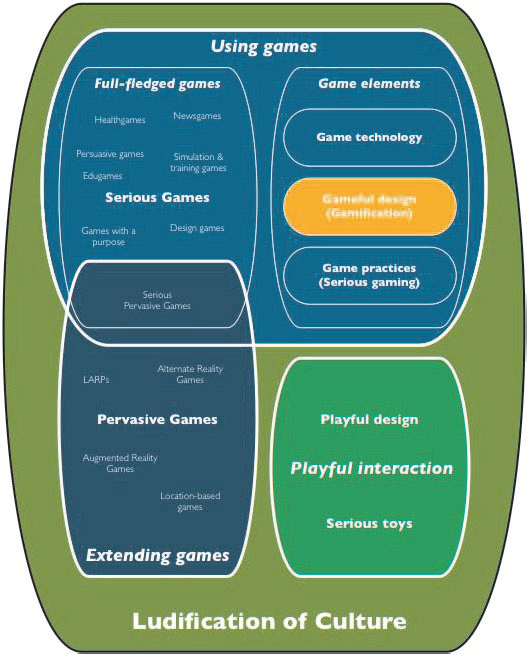
\includegraphics[width=80mm]{images/ch3_img02_gamification.png}
\caption{Gamification nach \cite{Deterding.2011}}
\label{img:ch3_img02_gamification}
\end{center}
\end{figure}
%
%\begin{figure}[H]
%\begin{center}
%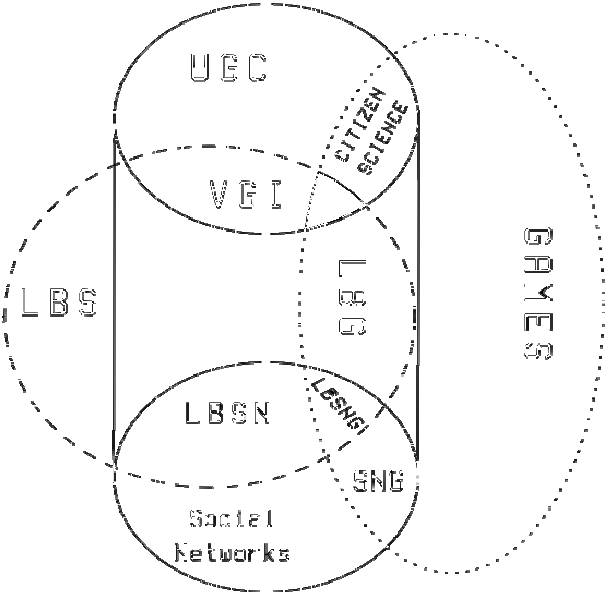
\includegraphics[width=80mm]{images/ch3_img01_LBG_SN_etc.png}
%\caption{Einordnung Definition}
%\label{img:ch3_img01_LBG_SN_etc}
%\end{center}
%\end{figure}

In der Literatur werden immer wieder die Elemente Points, Badges und Leaderboards (PBL) angesprochen. Diese dienen als Mittel um eine Gamification durchführen zu können. 
Points stellen Punkte dar, die verwendet werden um einen Fortschritt des einzelnen Spielers darzustellen. Dies sind zum Beispiel Meilen in Vielfliegerprogrammen oder Statuspunkte bei Bahn Bonus.
Bei Badges handelt es sich um Abzeichen, welche für bestimmte Erungenschaften an den Spieler vergeben werden. Ein Beispiel hierfür ist das Trainspotter Badget bei Foursquare, welches ausgestellt wird, wenn der Spieler in eine gewisse Anzahl von Bahnhöfen eingecheckt hat. Die Badges sollen einen gewissen Status gegenüber den restlichen Spielern suggestieren.
Leaderboards sind klassische Ranglisten. Diese dienen dazu einen Wettbwerb unter den Spielern zu erzeugen. Hierbei wird jedoch empfohlen nicht auf die klassische Top10 Liste, wie bei vielen Spielhallen Automaten zurückzugreifen. Stattdessen soll der Spieler zwischen anderen platziert werden, vorzugsweise sind die Spieler über und unter dem aktueller Spieler dessen Freunde (vgl. Foursquare). Dies verhindert, dass der Spieler von überhöhten Punktzahlen abgeschreckt wird.

\cite{Zichermann.2011} erweitern das Modell in dem es um weitere Aspekte ergänzen und mehr Struktur geben.
Sie pflegen den Begriff SAPS. Dieser unterteilt sich in Status, Access, Power und Stuff (SAPS).
Das bekannte PBL der Literatur wird unter Status zusammengefasst wie in nachfolgender Aufzählung zu sehen.

\begin{itemize}
      \item Status (Badges, Levels, Leaderboards)
      \item Access (early Access)
      \item Power (give power, e.g. modicum control over other players)
      \item Stuff (give a reward, try to prevent that the price gets known)
\end{itemize}

Bei Access handelt es sich um "Zugriff" zu exklusiven Dingen, welche man dem Spieler gewährt. Ein Beispiel hier für ist die Lufthansa Senator Lounge oder die DB Lounge.
Es kann sich aber auch um einen zeitlich verfrühten Zugriff auf ein Produkt oder Funktionen handeln.

Unter Power sind Mechaniken zu verstehen, welche es dem Spieler erlauben Einfluss - Macht - auf andere Spieler aus zu üben. Dies kann z.B. durch Moderationsrechte ab einem bestimmten Level realisiert werden. Foursquare realisiert dies durch Superuser.

Der letzte Punkt ist Stuff. Hierbei handelt es sich um Belohnungen die dem Spieler zuteilwerden. Klassischerweise handelte es sich hierbei z.B. um ein zusätzlich kostenloses Eis. Ziel ist es dem Spieler möglichst nicht einen konkreten monitären Gegenwert sehen zu lassen. D.h. dem Spieler soll es nicht ersichtlich sein wie viel der Reward wert ist. Ziel sollte es daher auch nicht sein einfach etwas kostenlos dem Spieler zu geben, sondern viel mehr etwas, was wiederum seinen Status unterstreicht.\\

Im Zuge der Gamification wird gerne der Begriff des \textit{Flow}-Zustandes aufgegriffen.
Hierbei handelt es sich um einen von \cite{Csikszentmihalyi.1991} eingeführten Begriff, bei dem es darum geht den Spieler zwischen einem Optimalen Zustand zwischen Angespannt heit und Langeweile zu halten. Hierbei soll auch basierend auf dessen Motivations- und dessen Erfahrungslevel ein inidividueller optimale Punkt erreicht werden.

(Flow Grafik)

\section{Geogames}
\label{subsec:S3_Geogames}

Game/Spiel:

According to  Katie  Salen  and  Eric  Zimmerman  (2004): "Magic circle"

Mobilegames
-games played on mobile devices (Bell et al. 2006)

Locationbased Games
games played in a location context
Kiefer et al. 2006, Benford et al. 2003
"Extending Cyberspace: Location Based Games Using Cellular Phones":
Rashid 2006

Geogames:
Schlieder et al. 2006

Pervasive Games

bluring the magic circle in "Montola, Markus. "Exploring the edge of the magic circle: Defining pervasive games." Proceedings of DAC. 2005."

"A pervasive game is agame that has one or more salient features that expand the 
contractual magie circle of play spatially, temporally, or socially. " @ Motola et al 2009

" This   definition   has   been   discussed   earlier  in   Montola   (2005)   and   in   Montola,   Waern,   and 
Nieuwdorp  (2006).  Staffan  Björk  (2007)  has  also  published  an  alternate version,  where  ambiguity 
of  interaction or  interface is  included  as  a  fourth  central  defining ceriterion." 

Can You See Me Now (CYSMN) (Flintham et al., 2003a)
GeoTicTacToe and CityPoker (see Schlieder et al. 2005a, Schlieder 2005b)
Human Pacman, realised by Choek et al. (2004)

Unterscheidung zwischen LBG, AR MR etc:

Concepts and Technologies for Pervasive Games (A reader for pervasive gaming research) (Hinske et al., 2007)

Es gibt viele verschiedene umgesetzte Spiele im Geogames/Pervasive Gaming Bereich

\section{Relokalisierungsansätze}

Generell was ist eine Location?
Wodurch wird diese definiert?


Literatur von KInf, sonst keine in diesem Umfeld.
Relocalisierungsansätze werden zwar angesprochen, z.B. in 
Exploring the Edge of the Magic Circle: 
Defining Pervasive Games 
Markus Montola 

es wird auf eventuelle Implikationen hingewiesen aber nicht im Detail weiter verfolgt.

Mannara 2012 ist ein erster Ansatz für ein Framework zu Relokalisierung von Spielfeldern basierend auf OSM Daten aber mit Fokus auf Eclipse EMF

\section{Verwendung offener Geodaten}
\label{subsec:S3_offeneGeodaten}

Hier: Was ist unter offen zu verstehen?

Es gibt zwei Bezugsquellen von öffentlichen Daten.
Zunächst die Daten welche von bestimmten Städten (vgl. Wien, Berlin, München) oder Ländern (Dänemark) den Bürgern zur Verfügung gestellt werden. Die Art, Qualität, sowie Umfang der Daten unterscheiden sich jedoch erheblich.

Eine zweite Option sind von offene (Geo-)Datenbanken, welche von privaten Personen durch Mapping oder externe lizenzierte Quellen zusammen gesammelt wurden. Eine dieser Datenbanken ist OpenStreetMap (OSM).


Haklay, Mordechai. "How good is volunteered geographical information? A comparative study of OpenStreetMap and Ordnance Survey datasets." Environment and planning. B, Planning \& design 37.4 (2010): 682.

\&

"Quality Assessment of the French OpenStreetMap Dataset" Girres et al. (2010)

Ergebnis:

Qualität der Daten von OSM hat seit dem Start (2004) enorm zugenommen, je nach Land besteht eine höhere Abdeckungsrate. Zur Zeit gibt es ca 20.000 aktive Mapper.

Mapping in Städten deutlich genauer wie "auf dem Land/außerhalb".  avg. distance ~1 vs ~30m.

Es gibt eine generelle Ungenauigkeit bei den Namen der Objekte.

Logische Konsistenz im Modell von OSM nicht verhanden.

Hecht 2013:
-Abdeckung/Coverage relativ gering, allerdings Genauigkeit proportional zu Stadtgröße

Pfoser et al. 2013:
-zwar teilweise gernige coverage, aber sehr hohe Klassifikationsrate, bei dennoch hoher Fehlerate von bis zu 23%
